\documentclass[10pt]{amsart}
\usepackage[margin=1.4in]{geometry}
\usepackage{amssymb,amsmath,enumitem,url}
\usepackage{graphicx,subfig}
\graphicspath{ {./images/} }

\newcommand{\D}{\mathrm{d}}
\newcommand{\I}{\mathrm{i}}
\DeclareMathOperator{\E}{e}
\DeclareMathOperator{\OO}{O}
\DeclareMathOperator{\oo}{o}
\DeclareMathOperator{\erfc}{erfc}
\DeclareMathOperator{\real}{Re}
\DeclareMathOperator{\imag}{Im}
\usepackage{tikz}
\usepackage[framemethod=tikz]{mdframed}
\theoremstyle{nonumberplain}

\mdtheorem[innertopmargin=-5pt]{sol}{Solution}
%\newmdtheoremenv[innertopmargin=-5pt]{sol}{Solution}

\begin{document}
\pagestyle{empty}

\newcommand{\mline}{\vspace{.2in}\hrule\vspace{.2in}}

\noindent
\text{Hunter Lybbert} \\
\text{Student ID: 2426454} \\
\text{01-23-25} \\
\text{AMATH 502} \\
% header containing your name, student number, due date, course, and the homework number as a title.

\title{\bf {Homework 2} }


\maketitle
\noindent
Exercises come from \textit{Nonlinear Dynamics and Chaos by Steven H. Strogatz}
\mline
\begin{enumerate}[label={\bf {\arabic*}:}]
\item 2.6.1 Explain this paradox: a simple harmonic oscillator $m\ddot {x} = -k x$ is a system which oscillates in one dimension (along the $x$-axis). But the text says one-dimensional systems can't oscillate. \\

\noindent
\textit{Solution:} \\
Not a formal method of finding a solution but I can see that if $x = \sin \left(  \frac k m t \right)$ then
\begin{align*}
\dot x &= \frac k m \cos \left(  \frac k m t \right) \\
\ddot x &= - \frac {k^2} {m^2} \sin \left(  \frac k m t \right) \\
\ddot x &= - \frac {k^2} {m^2} x \\
m^2\ddot x &= - k^2 x
\end{align*}
Therefore to adjust the constants $k$ and $m$ so they agree with the original solution we need to actually have $x = \sin \big(  \sqrt {k/m} \: t \big)$.
Furthermore, we could similarly have arrived at a similar solution with $x = \cos \big(  \sqrt {k/m} \: t \big)$.
Therefore, we have
$$x = c_1 \sin \big(  \sqrt {k/m} \: t \big) + c_2 \cos \big(  \sqrt {k/m} \: t \big).$$
Now setting all this aside, we have to look more closely at the original system.
Since this is a second derivative in $x$, we are actually implicitly depending on the position and velocity the value of $x$ and it's first derivative.
Therefore this is not actually a first order system and thus is not a contradiction to the statements in the text about first order systems.
\qed \\

\newpage

\item 3.1.1 $\dot x = 1 + rx + x^2$ \\
Sketch all the qualitatively different vector fields that occur as $r$ is varied.
Show that a saddle-node bifurcation occurs at a critical value of $r$, to be determined.
Finally sketch the bifurcation diagram of fixed points $x^*$ vs. $r$. \\

\noindent
\textit{Solution:} \\
Well we know that we have fixed points at
$$x = \frac {-r \pm \sqrt {r^2 - 4}}{2}$$
which implies there are no fixed points when $|r| < 2$, a single fixed point when $r = \pm 2$, and two fixed points when $|r| > 2$.

\begin{figure}[h]
	\centering
	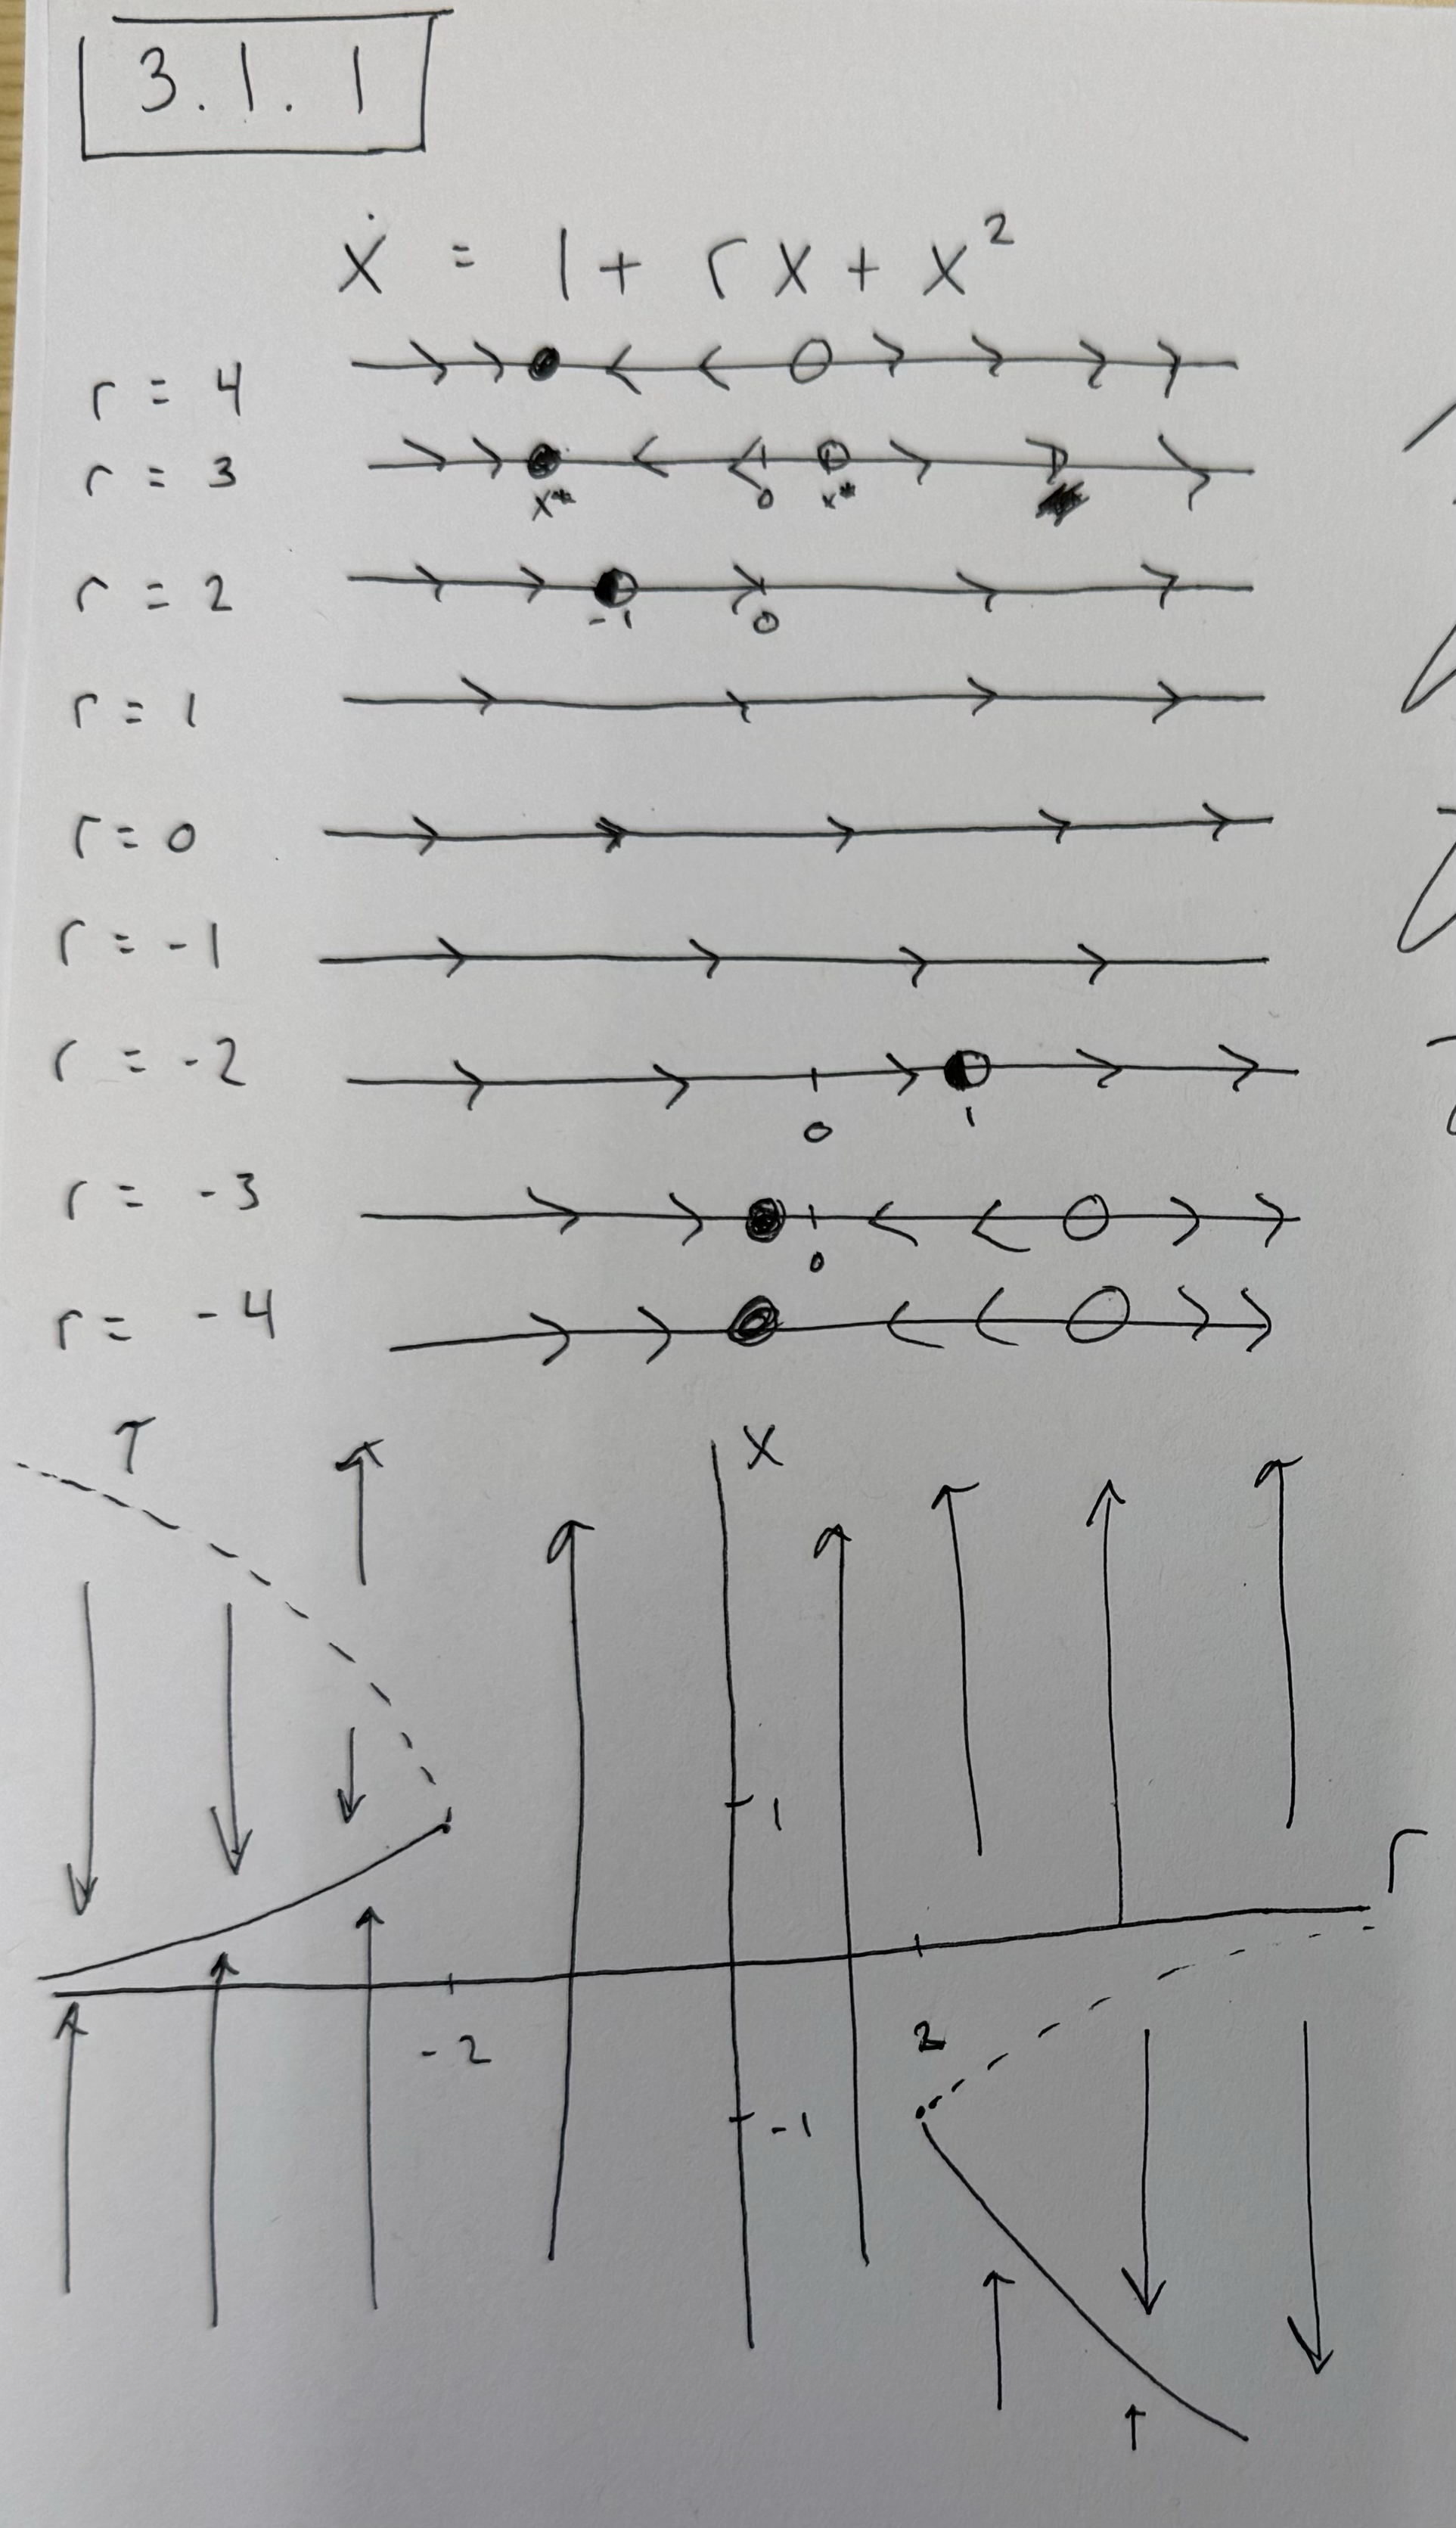
\includegraphics[height=.5\textwidth]{3_1_1.png}
 	\caption{We have sketched the vector field of $x$ for various values of $r$. Additionally we have sketched the bifurcation diagram.}\label{fig:f1}
\end{figure}
\qed \\

\newpage

\item 3.1.5 (Unusual bifurcations) In discussing the normal form of the saddle-node bifurcation, we mentioned the assumption that $a = \left. \partial f / \partial r \right|_{(x^*, r_c)} \neq 0.$
To see what can happen if $a = \left. \partial f / \partial r \right|_{(x^*, r_c)} = 0$, sketch the vector fields for the following examples, and then plot the fixed points as a function of $r$. \\


\begin{enumerate}
\item $\dot x = r^2 - x^2$ 
\textit{Solution:} \\
We know that the rhs is equal to 0 when $x^* = \pm r$. So we plot a series of the vector fields for various values of $r$. See Figure \ref{fig:f2}.

\begin{figure}[h]
	\centering
	\includegraphics[height=2in]{3_1_5_a.png}
 	\caption{We have sketched the vector field of $x$ for various values of $r$. Additionally we have sketched the bifurcation diagram.}\label{fig:f2}
\end{figure}

\item $\dot x = r^2 + x^2$ \\
\textit{Solution:} In this instance there is only one fixed point when $r = 0$ and no fixed points for any other value of $r$. See Figure \ref{fig:f3}.

\begin{figure}[h]
	\centering
	\includegraphics[height=2in]{3_1_5_b.png}
 	\caption{We have sketched the vector field of $x$ for various values of $r$. Additionally we have sketched the bifurcation diagram.}\label{fig:f3}
\end{figure}
\end{enumerate}

\qed \\ 

\newpage


\item 3.2.3 $\dot x = x - rx(1 - x)$ \\
Sketch all the qualitatively different vector fields that occur as $r$ is varied.
Show that transcritical bifurcation occurs at a critical value of $r$, to be determined.
Finally, sketch the bifurcation diagram of fixed points $x^*$ vs. $r$. \\

\noindent
\textit{Solution:} \\
Notice we have
\begin{align*}
\dot x &= x - rx(1 - x) \\
\dot x &= (1 - r)x(1 - x)
\end{align*}
Therefore we have fixed points at $x^* = 0, 1$ independent of values of $r$.
However, if $r = 1$, then $\dot x = 0$ trivially

\begin{figure}[h]
	\centering
	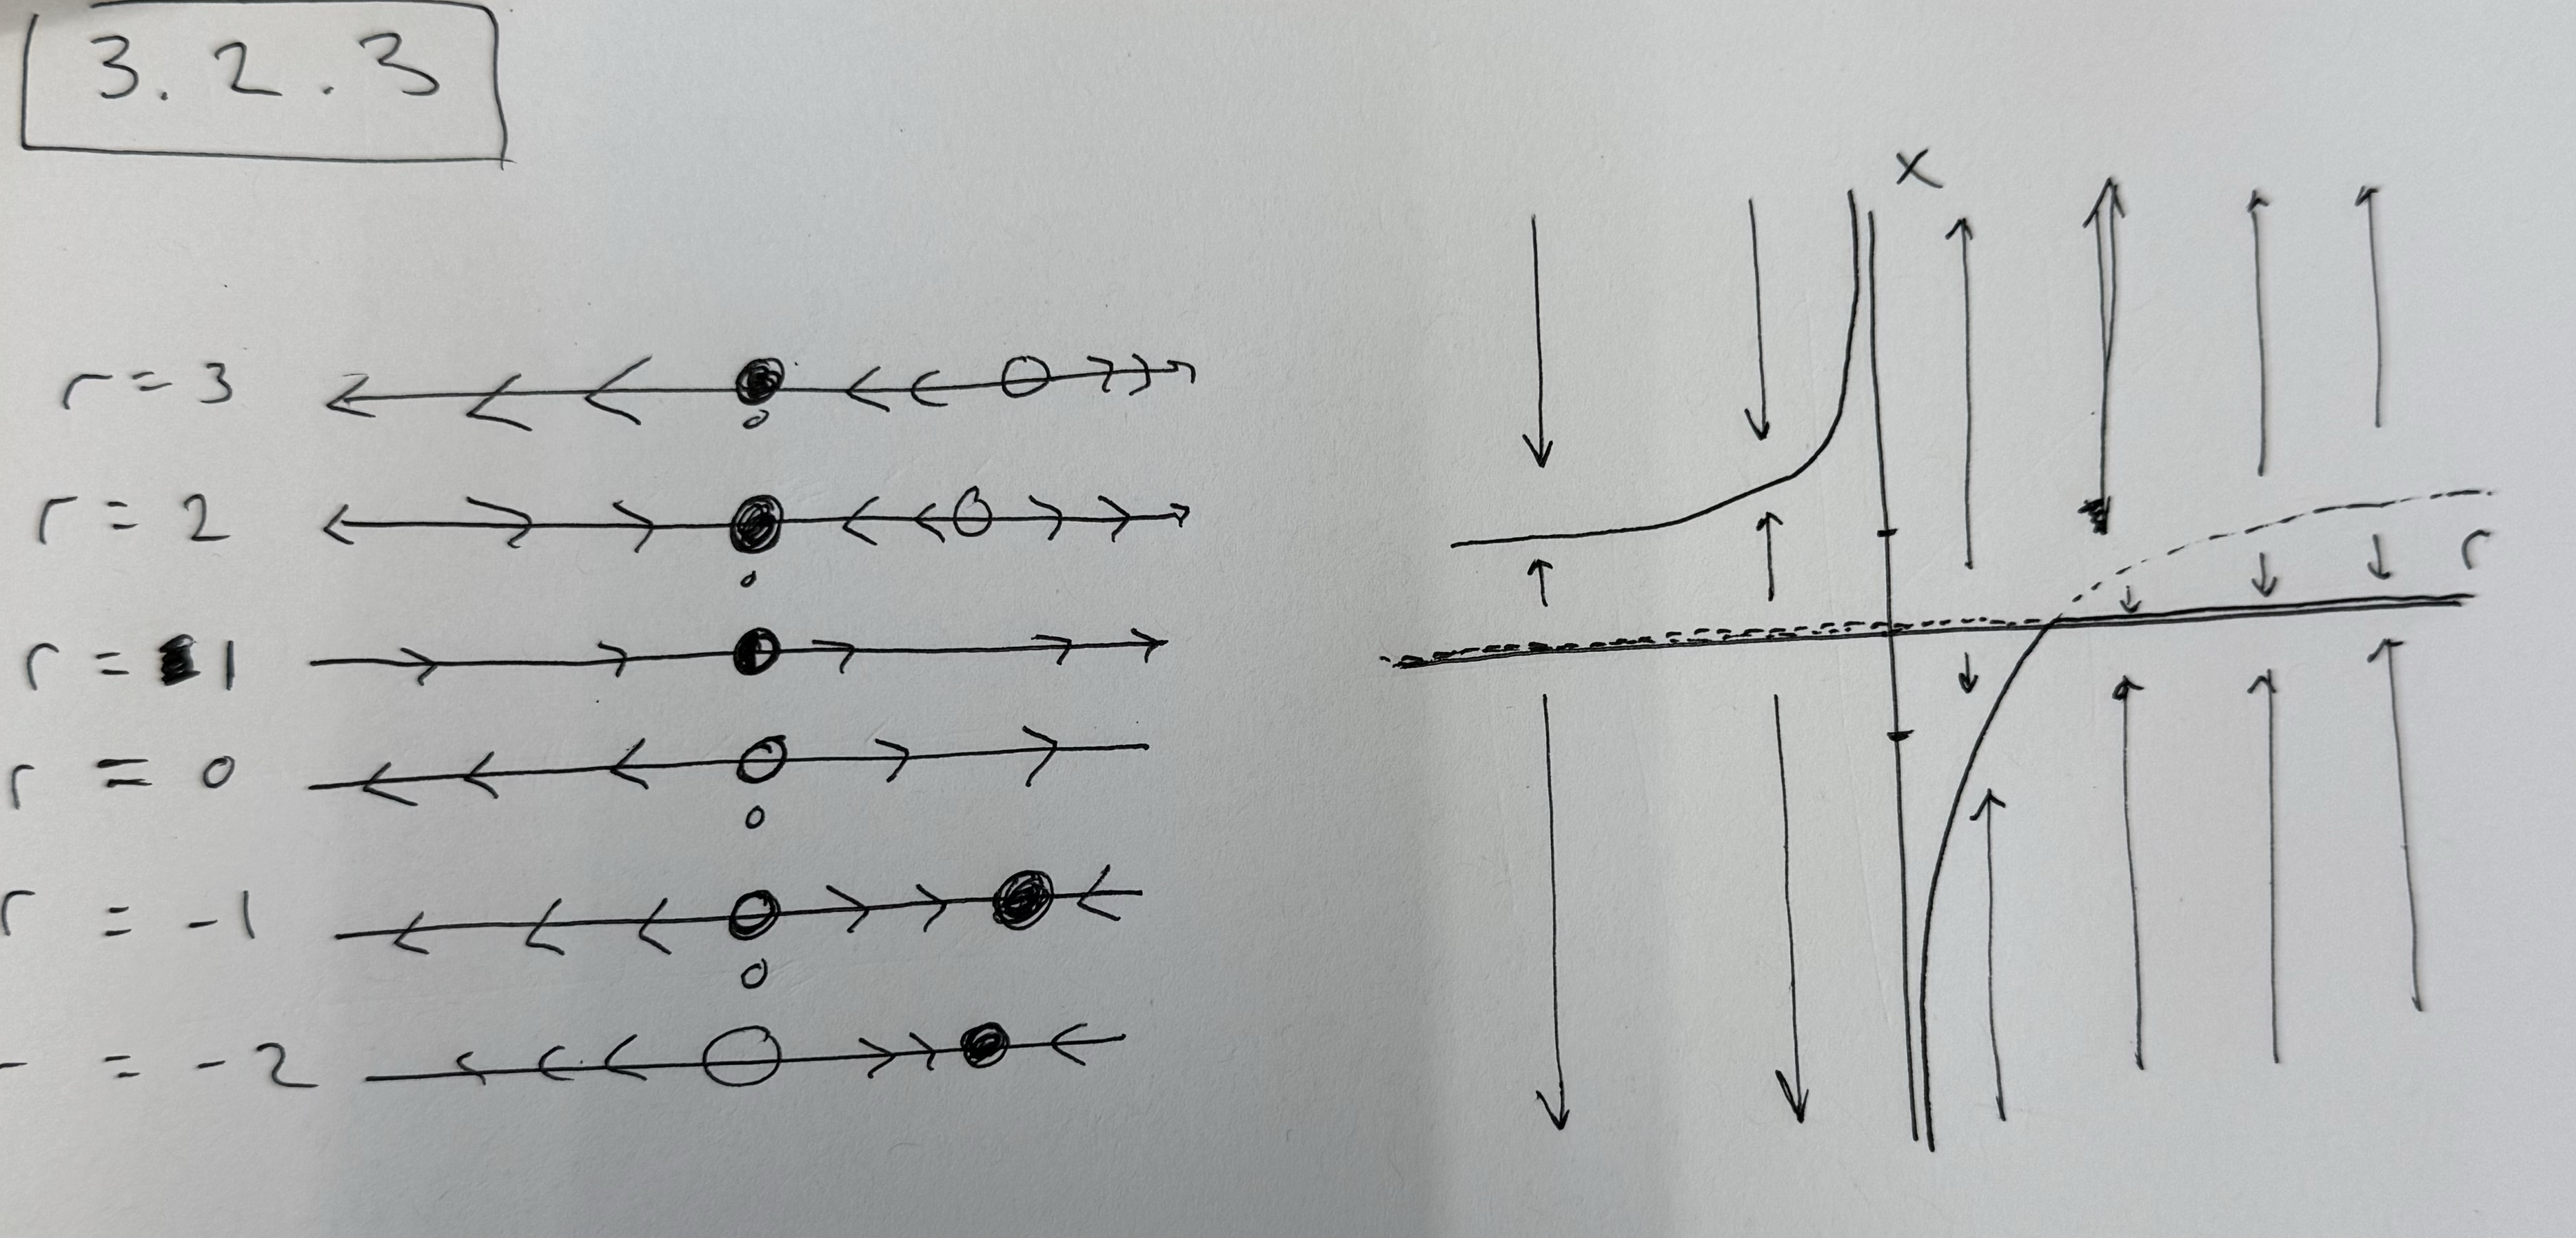
\includegraphics[height=2in]{3_2_3.png}
 	\caption{We have sketched the vector field of $x$ for various values of $r$. Additionally we have sketched the bifurcation diagram.}\label{fig:f4}
\end{figure}

\qed \\ 

\newpage

\item 3.4.11 (An interesting bifurcation diagram) Consider $\dot x = rx - \sin x$ \\
\begin{enumerate}

\item For the case $r = 0$, find and classify all the fixed points, and sketch the vector field. \\

\noindent
\textit{Solution:} \\
When $r = 0$, then we have $\dot x = - \sin x$.
Therefore we have fixed points at $x^* = k\pi$ for $k \in \mathbb Z$.
See Figure \ref{fig:f5} below. \\
\qed \\

\item Show that when $r > 1$, there is only one fixed point.
What kind of fixed point is it? \\

\noindent
\textit{Solution:} \\
There is only one fixed point at $x^* = 0$ and it is unstable.
See Figure \ref{fig:f5} below. \\
\qed \\

\item As $r$ decreases from $\infty$ to $0$, classify \textit{all} the bifurcations that occur. \\

\noindent
\textit{Solution:} \\
As $r$ decreases from $\infty$ to $0$ there is only one fixed point until $r < 1$ then rapidly more fixed points and bifurcations occur.
Additionally when $r < 1$ the stability of the fixed point at 0 changes and becomes stable.
They are added in pairs on both sides of 0 each pair alternating from stable and unstable. \\
\qed \\

\item For $0 < r << 1$, find an approximate formula for values of $r$ at which bifurcations occur. \\

\noindent
\textit{Solution:} \\
We begin by looking at when $rx - \sin x = 0$ as well as when $r - \cos x = 0$.
These in turn give us $r = \cos x$ and $r = \frac {\sin x}{x}$.
Furthermore, if $r$ is really small and nearly 0, then we basically have fixed points when $\cos x = 0$ in other words at $x^* = \frac {\pi}{2} + 2 \pi k$ for $k \in \mathbb Z$.
Combining this with the information we have from before we then have
$$
r = \frac {\sin \left( \frac {\pi}{2} + 2 \pi k\right)}{\frac {\pi}{2} + 2 \pi k}
= \frac{1}{\frac {\pi}{2} + 2 \pi k}.
$$
\qed \\

\item Now classify all the bifurcations that occur as $r$ decreases from 0 to $-\infty$. \\

\noindent
\textit{Solution:} \\
Similar to going from $\infty$ to $0$ we have only one stable fixed point at $x^* = 0$ as $r$ goes from $-\infty$ to some small negative value approximately close to $r \approx -.224$ then as $r$ get's closer and closer to $0$ additional fixed points are added to the system.
They are added in a similar manner as in part c) in pairs and alternating stability as you go out to negative and positive infinity. \\
\qed \\

\item Plot the Bifurcation diagram for $-\infty < r < \infty$, and indicate the stability of the various branches of fixed points. \\

\noindent
\textit{Solution:} \\
See Figure \ref{fig:f5}, note the dotted and solid lines indicating the stability of the branches of fixed points.

\begin{figure}[h]
	\centering
	\includegraphics[height=2in]{3_4_11.png}
 	\caption{We have sketched the vector field of $x$ for various values of $r$. Additionally we have sketched the bifurcation diagram.}\label{fig:f5}
\end{figure}

\end{enumerate}

\qed \\

\newpage

\item 3.5.8 (Nondimensionalizing the subcritical pitchfork) The first-order system $\dot u = au + bu^3 - c u^5$, where $b, c > 0$, has a subcritical pitchfork bifurcation at $a = 0$.
Show that this equation can be rewritten as
$$\frac {dx}{d\tau} = r x + x^3 - x^5$$
where $x = u/U$, $\tau = t/T$, and $U$, $T$, and $r$ are to be determined in terms of $a$, $b$, and $c$. \\

\noindent
\textit{Solution:} \\
We are using the substitutions provided so we can also note that they result in $U dx = du$ and $T d\tau = d t$.
Then we have 
\begin{align}
\dot u &= au + bu^3 - c u^5 \nonumber \\
\frac {du}{dt} &= au + bu^3 - c u^5 \nonumber \\
\frac {Udx}{Td\tau} &= a(Ux) + b(Ux)^3 - c (Ux)^5 \nonumber \\
\frac {dx}{d\tau} &= Tax + TbU^2x^3 - TcU^4x^5.
\label{eq:eq1}
\end{align}
In order for this to give us the final equation we are looking for we need the following to all hold
\begin{align*}
Ta = r, \quad
TbU^2 = 1, \quad
TcU^4 = 1.
\end{align*}
Let's solve these so we have $U$, $T$, and $r$ in terms of $a$, $b$, and $c$.
Beginning with the second equation we have $T = 1/bU^2$ and plugging that into the third equation we get
$\frac 1 {bU^2} cU^4 = 1$ then simplifying gives us 
\begin{align*}
\frac c b U^2 &= 1 \\
U^2 &= \frac b c \\
U &= \sqrt{\frac b c}.
\end{align*}
Thus we also have
\begin{align*}
T &= \frac 1 {bU^2} = \frac 1 {b \frac b c} = \frac c {b^2}.
\end{align*}
Hence
$$
T = \frac c {b^2}, \quad
U = \sqrt{\frac b c}, \quad
r = \frac {ac} {b^2}.
$$
Finally we can combine this with \eqref{eq:eq1} to see
\begin{align*}
\dot u &= au + bu^3 - c u^5 \\
\frac {dx}{d\tau} &= Tax + TbU^2x^3 - TcU^4x^5 \\
\frac {dx}{d\tau} &= \frac {ac} {b^2}ax + \frac{cb} {b^2} \sqrt{\frac b c}^2x^3 - \frac {c^2} {b^2} \sqrt{\frac b c}^4x^5 \\
\frac {dx}{d\tau} &= r x + x^3 - x^5.
\end{align*} \qed \\

\newpage

\item 3.7.3 (A model of a fishery) The equation
$$\dot N = rN\left( 1 - \frac N K \right) - H$$
provides an extremely simple model of a fishery.
In the absence of fishing, the population is assumed to grow logistically. 
The effects of fishing are modeled by the term $-H$, which says that fish are caught or ``harvested" at a constant rate $H > 0$, independent of their population $N$.
(This assumes that the fisherman aren't worried about fishing the population dry--they simply catch the same number of fish every day.) \\

\begin{enumerate}

\item Show that the system can be rewritten in dimensionless form as 
$$
\frac {dx}{d\tau} = x(1 - x) - h
$$
for suitably defined dimensionless quantities $x$, $\tau$, and $h$ \\

\noindent
\textit{Solution:} \\
Let's use the substitutions  $Mx = N$ and $T\tau = t$ and their derivative forms $Mdx = dN$ and $Td\tau = dt$.
Now we can use these as follows
\begin{align*}
\dot N &= rN\left( 1 - \frac N K \right) - H \\
\frac {dN}{dt} &= rN\left( 1 - \frac N K \right) - H \\
\frac {Mdx}{Td\tau} &= rMx\left( 1 - \frac {Mx} K \right) - H \\
\frac {dx}{d\tau} &= T rx\left( 1 - \frac {Mx} K \right) - \frac{TH}M.
\end{align*}
Then we need the following to hold
$$Tr = 1, \quad \frac M K = 1, \quad \frac {TH} M = h.$$
This implies we have to choose $M = K$, $T = \frac 1 r$, and $h = \frac H {Kr}$.
Therefore,
\begin{align*}
\frac {dx}{d\tau} &= T rx\left( 1 - \frac {Mx} K \right) - \frac{TH}M \\
\frac {dx}{d\tau} &= \frac 1 r rx\left( 1 - \frac {Kx} K \right) - \frac H {Kr} \\
\frac {dx}{d\tau} &= x\left( 1 - x \right) - h
\end{align*}
\qed \\

\newpage

\item Plot the vector field for different values of $h$ \\

\noindent
\textit{Solution:} \\
Notice in this form we have fixed points at
$$x^* = \frac {-1 \pm \sqrt{1 - 4h}}{-2} = \frac {1 \mp \sqrt{1 - 4h}}{2}.$$
In Figure \ref{fig:f6} we can see the different vector fields for various values of $h$

\begin{figure}[h]
	\centering
	\includegraphics[height=2in]{3_7_3.png}
 	\caption{We have sketched the vector field of $x$ for various values of $h$.}\label{fig:f6}
\end{figure} \qed \\

\item Show that a bifurcation occurs at a certain value of $h_c$, and classify this bifurcation. \\

\noindent
\textit{Solution:} The bifurcation occurs at $h_c = \frac 1 4$.
And it is a saddle node bifurcation.
For further evidence, please refer to Figure \ref{fig:f6}.
\qed \\

\item Discuss the long-term behavior of the fish population for $h < h_c$ and $h > h_c$. 
Give the biological interpretation in each case. \\

\noindent
\textit{Solution:} 
For $h > h_c$ we would have overfishing or fishing at a rate faster than they can be born or replenished and thus would result in an extinction.
Furthermore, if $h < h_c$ the fishing rate and birth rates would arrive to an equilibrium of sorts and reach a steady state solution at $x^* = \frac {1 + \sqrt{1 - 4h}}{2}$. \\
\qed \\

\end{enumerate}

\end{enumerate}

\end{document}

%%% Local Variables:
%%% mode: latex
%%% TeX-master: t
%%% End:
